\section{Part 2 - Dataset Analysis}

In this section we show the details and results of our dataset analysis and how it relates
to our research objectives discussed in Part 1.

\subsection{Dataset demographics}

In "Sub-objective 1", we explained why understanding the dataset demographics is essential to ensure
our prediction model does not suffer from any biases.

We start by counting the number of patients with and without reported heart disease. Table \ref{demographics-target-percent}
shows the percentage of patients with and without heart disease. Figure \ref{demographics-target-count} shows
the total number of patients with and without a heart condition.

\small
\begin{tabularx}{\linewidth}{ | X | X |}
    \caption{Distribution of patients with and without a heart condition}\label{demographics-target-percent} \\
    \hline
    \textbf{Target} & \textbf{Count}\\
    \hline
    No heart disease & 42\% \\
    \hline
    Heart disease & 58\% \\
    \hline
\end{tabularx}
\normalsize

\begin{figure}
    \caption{Number of patients with and without a heart condition}\label{demographics-target-count}
    \centering
    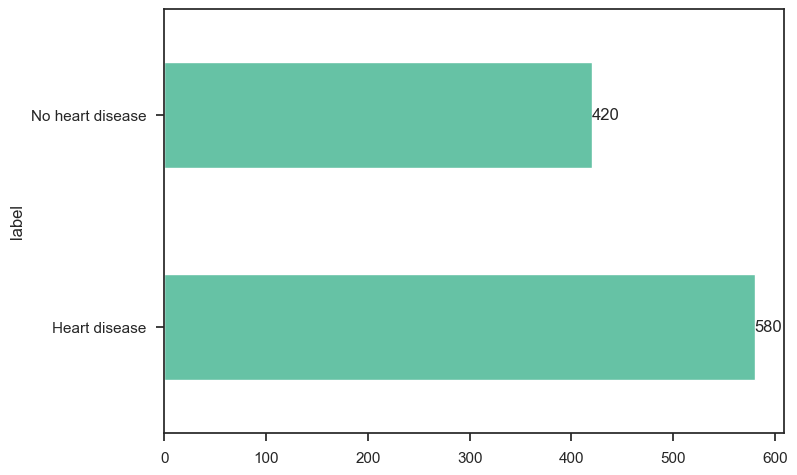
\includegraphics[width=\linewidth]{media/demographics-01-target.png}
\end{figure}

These values show that the dataset \textbf{is well balanced between assigned labels} (i.e. classification). This
is important to ensure that our prediction model has enough training data.

\subsubsection{Gender demographics}

To identify potential gender bias and ensure that our prediction model is accurate for any gender, we analyse
the distribution of data across genders.

Figure \ref{demographics-gender-target-count} shows that there are more than double the amount of male patients
compare to female patients. Table \ref{demographics-gender-percent} shows that the number of female patients is
only 23\% of the total. This \textbf{could point to a lower incidence of heart-related conditions in the female population},
but we cannot confirm it without gathering more details about the recruitment strategy for the dataset.
    
\begin{figure}
    \caption{Number of patients of each gender grouped by class}\label{demographics-gender-target-count}
    \centering
    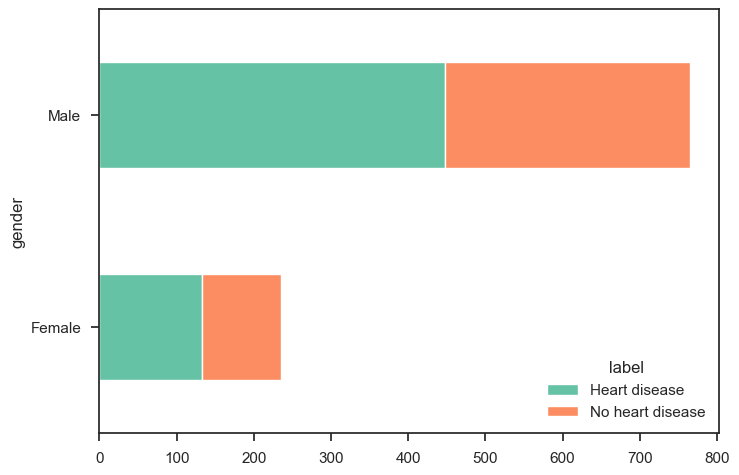
\includegraphics[width=\linewidth]{media/demographics-03-gender-target-count.png}
\end{figure}

\small
\begin{tabularx}{\linewidth}{ | X | X |}
    \caption{Distribution of patients of each gender}\label{demographics-gender-percent} \\
    \hline
    \textbf{Gender} & \textbf{Percentage}\\
    \hline
    Female & 23\% \\
    \hline
    Male & 77\% \\
    \hline
\end{tabularx}
\normalsize

Assuming that the bias towards male patients is not representative of disease incidence, we must at least
ensure that the distribution of patients with disease is constant across genders, so that the prediction
model will not tend to disproportionally apply a specific class to a whole gender.

Figure \ref{demographics-gender-target-percent} shows the \textbf{distribution of patients with disease across genders},
and confirms that indeed the \textbf{distribution is balanced}.

\begin{figure}
    \caption{Distribution of patients of each gender grouped by class}\label{demographics-gender-target-percent}
    \centering
    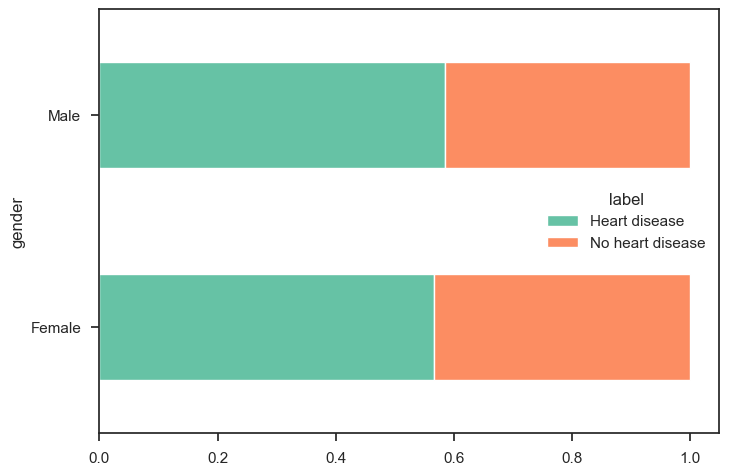
\includegraphics[width=\linewidth]{media/demographics-04-gender-target-percentage.png}
\end{figure}

In the next section we will analyse the age demographics of the dataset, but we must also ensure that
there is an even number of patients of each gender across the different age groups. 

Figure \ref{demographics-gender-agegroup-count} shows the number of patients in each age group grouped by
gender. Although there are small variations between the female and the male populations, the
\textbf{distribution is balanced, there are roughly an equal number of patients across each age group when
grouping by gender.}

\begin{figure}
    \caption{Number of patients of each gender across age groups}\label{demographics-gender-agegroup-count}
    \centering
    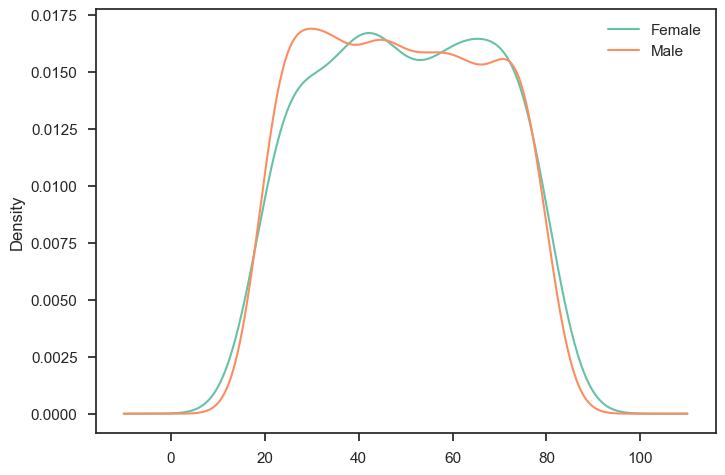
\includegraphics[width=\linewidth]{media/demographics-02-gender-age.png}
\end{figure}

\subsubsection{Age demographics}

In the same way we have checked the gender demographics, we must also validate the age demographics to ensure that
our result prediction model produces equally accurate results across the age spectrum.

Figure \ref{demographics-agegroup-target-percent} shows the distribution of patients of each age group grouping by class
(with and without heart disease). It is visually apparent that this distribution is also consistent across ages,
\textbf{presumably the recruitment criteria ensured that there would be a balanced distribution across genders and ages} for both
ill and healthy patients.

\begin{figure}
    \caption{Distribution of patients of each age group grouped by class}\label{demographics-agegroup-target-percent}
    \centering
    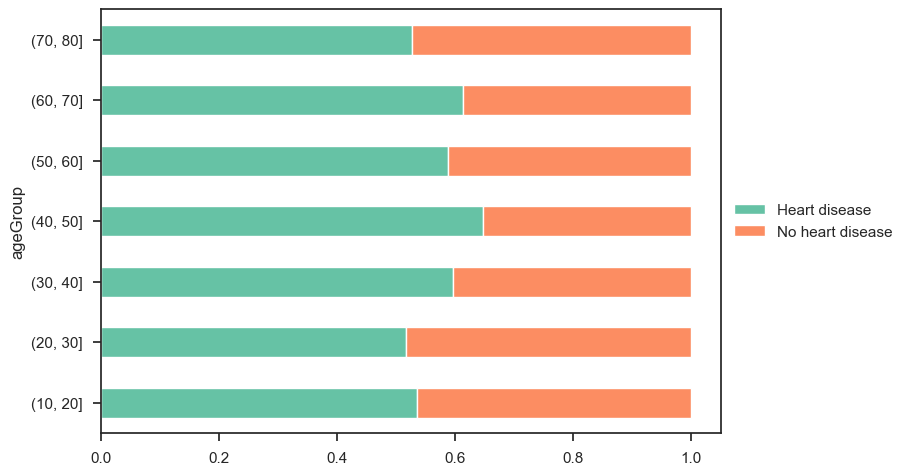
\includegraphics[width=\linewidth]{media/demographics-05-agegroup-target-percentage.png}
\end{figure}


\subsection{Frequency Analysis}

In this section we show the result of the frequency analysis of the categorical features. This analysis allows us to
better understand the dataset and to speculate about correlation between each feature and the presence of
heart disease.

\subsubsection{Feature: Number of major vessels}

This feature represents the number of major vessels visible through a fluoroscopy. Research \cite{Fluoroscopy} shows that
there is a strong correlation between the number of coloured vessels and the presence of cardiovascular diseases.
The fewer visible vessels, the most likely it is that the patient suffers from a heart condition.

Nonetheless, our data seems to suggest the opposite. Figures \ref{frequency-vessel-gender-percent} and \ref{frequency-vessel-age-percent}
show a visible relationship between the presence of disease an an increase number of visible major vessels.

It is not clear where the discrepancy between the dataset and the recent studies comes from, but our prediction
model should still be effective as long as the distribution is simply reversed.

\begin{figure}
    \caption{Distribution of the number of major vessels visible grouping by gender}\label{frequency-vessel-gender-percent}
    \centering
    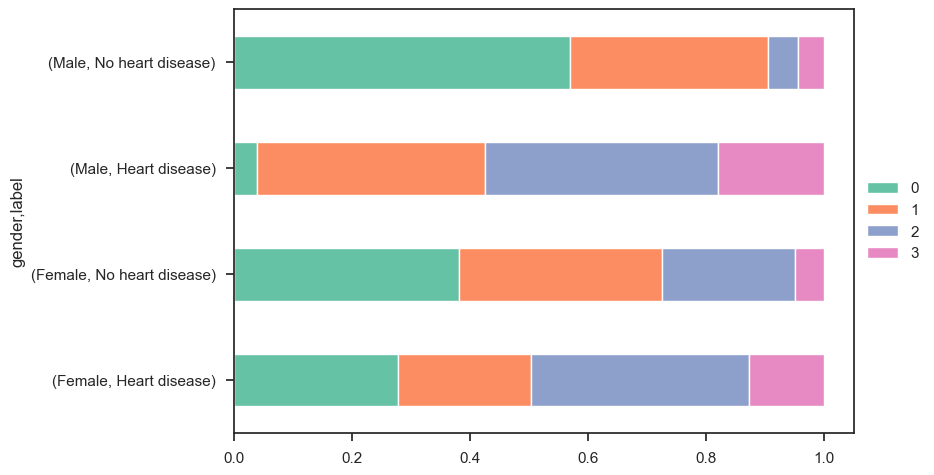
\includegraphics[width=\linewidth]{media/frequency-01-gender-vessels.png}
\end{figure}

\begin{figure}
    \caption{Distribution of the number of major vessels visible grouping by age groups}\label{frequency-vessel-age-percent}
    \centering
    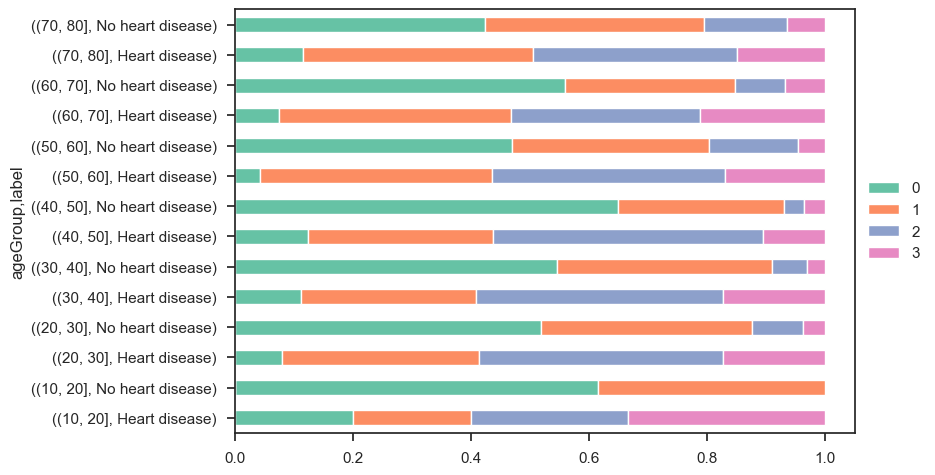
\includegraphics[width=\linewidth]{media/frequency-02-agegroup-vessels.png}
\end{figure}

\subsubsection{Feature: Slope}

This feature represents the shape of the slope at the exercise peak. In figures \ref{frequency-slope-gender-percent}
and \ref{frequency-slope-agegroup-percent} we can see that there is a relationship between the inclination of the slope
and the presence of cardiovascular disease. These observations are substantiated by existing research \cite{Fluoroscopy}.

\begin{figure}
    \caption{Distribution of slope classification grouping by gender}\label{frequency-slope-gender-percent}
    \centering
    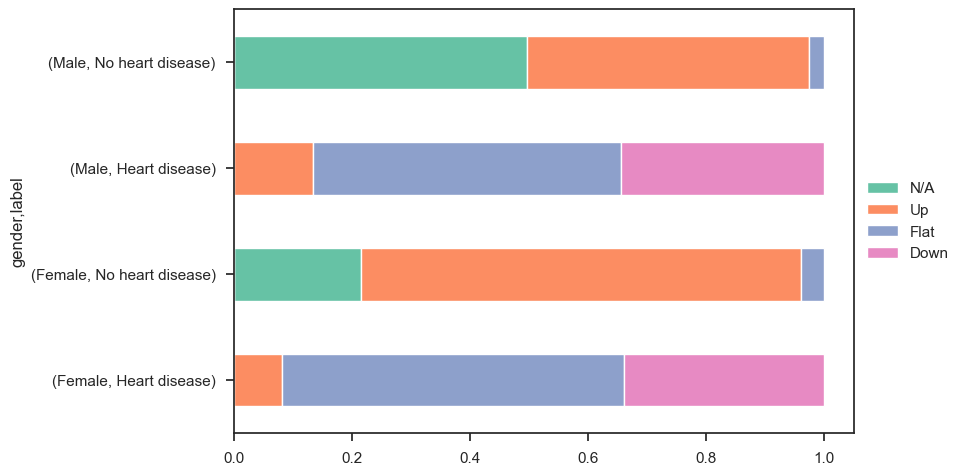
\includegraphics[width=\linewidth]{media/frequency-03-gender-slope.png}
\end{figure}

\begin{figure}
    \caption{Distribution of slope classification grouping by age groups}\label{frequency-slope-agegroup-percent}
    \centering
    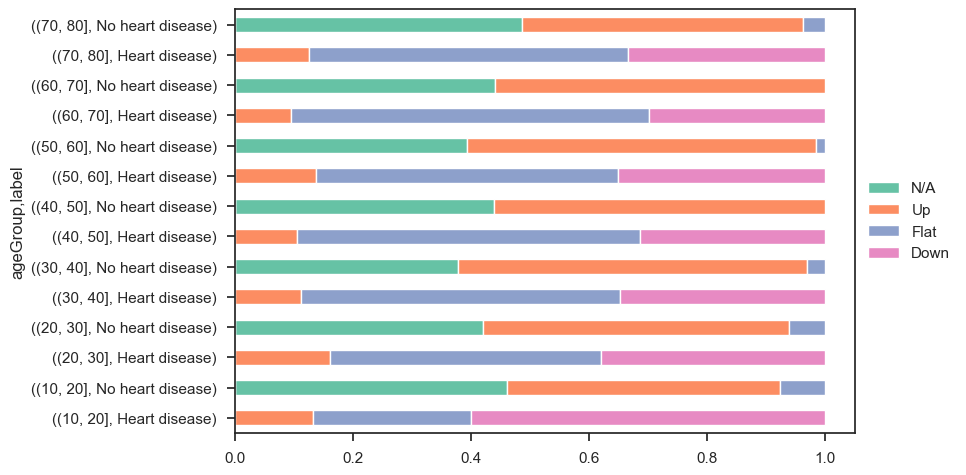
\includegraphics[width=\linewidth]{media/frequency-04-agegroup-slope.png}
\end{figure}

Healthy patients have either an upwards slope or a flat slope, patients with a heart disease are more likely to show
a downwards slope.

Note that there are a substantial amount of samples that don't have a valid classification value for this feature.

\subsubsection{Feature: Resting electrocardiogram results}

This feature is a classification of the results of a ECG while the patient is at rest. Figures \ref{frequency-ecg-gender-percent}
and \ref{frequency-ecg-agegroup-percent} show what is already intuitive, an abnormal ECG result correlates with
the presence of heart conditions across genders and ages.

\begin{figure}
    \caption{Distribution of resting ECG results classification grouping by gender}\label{frequency-ecg-gender-percent}
    \centering
    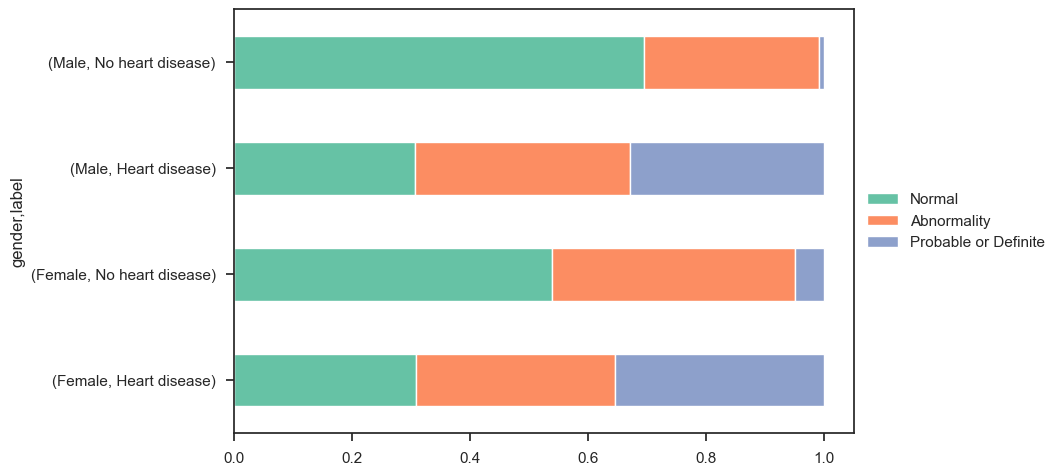
\includegraphics[width=\linewidth]{media/frequency-05-gender-ecg.png}
\end{figure}

\begin{figure}
    \caption{Distribution of resting ECG results classification grouping by age groups}\label{frequency-ecg-agegroup-percent}
    \centering
    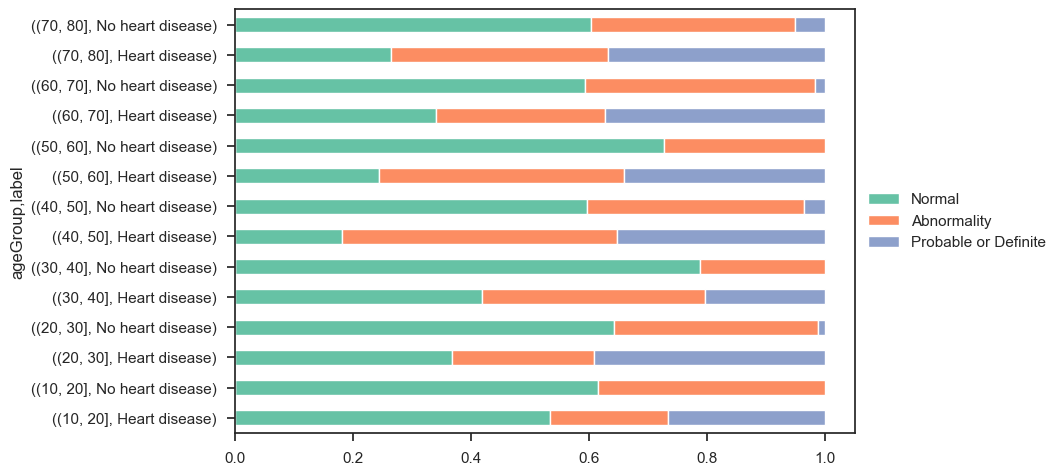
\includegraphics[width=\linewidth]{media/frequency-06-agegroup-ecg.png}
\end{figure}

There are, nonetheless, a couple of observations worth noting. Firstly, there are patients that are not affected
by any heart condition, and yet show abnormal or even strong signs of disease in the ECG. Lastly, female patients
seem to be more likely to show probable signs of disease in the ECG even when they are healthy.

\subsubsection{Feature: Fasting blood sugar}

This feature classifies the levels of blood sugar measured while the patient is fasting. The classification is based
on a threshold of 120 mg/dl.

Once more, we see certain correlation in figures \ref{frequency-bloodsugar-gender-percent} and
\ref{frequency-bloodsugar-agegroup-percent}.

\begin{figure}
    \caption{Distribution of blood sugar level classification grouping by gender}\label{frequency-bloodsugar-gender-percent}
    \centering
    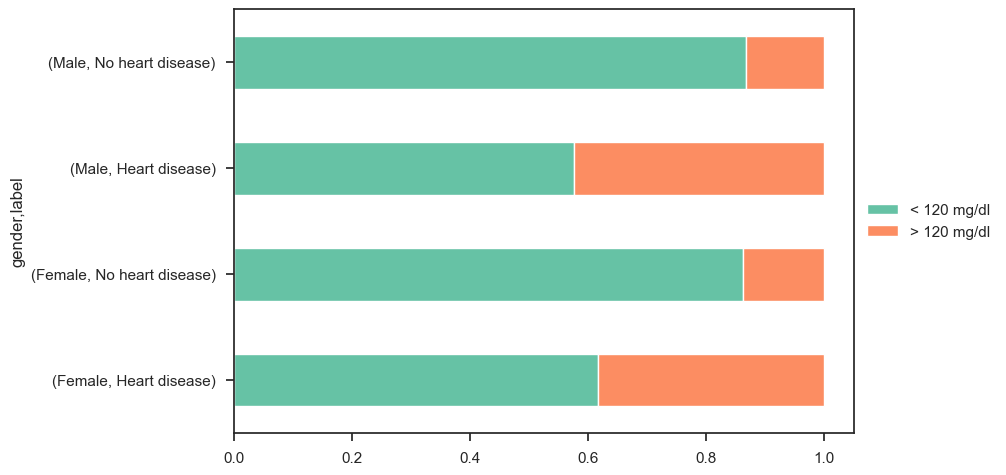
\includegraphics[width=\linewidth]{media/frequency-07-gender-bloodsugar.png}
\end{figure}

\begin{figure}
    \caption{Distribution of blood sugar level classification grouping by age groups}\label{frequency-bloodsugar-agegroup-percent}
    \centering
    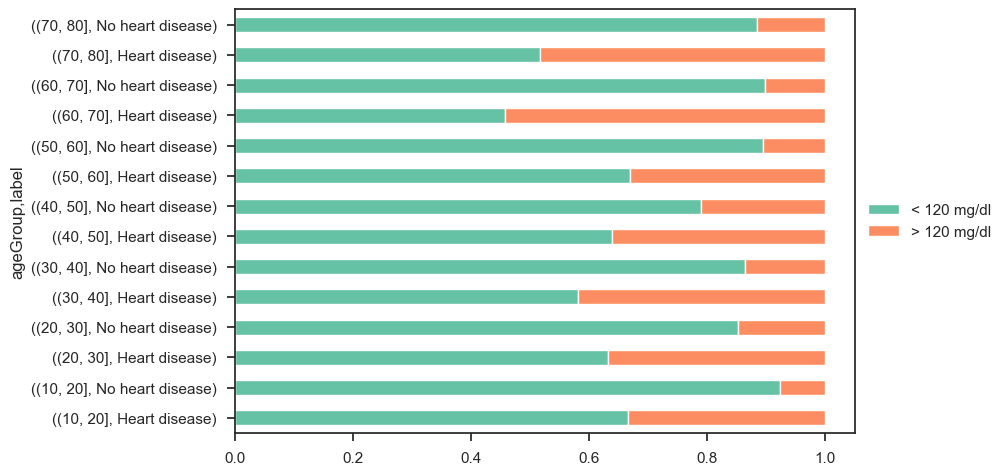
\includegraphics[width=\linewidth]{media/frequency-08-agegroup-bloodsugar.png}
\end{figure}

An interesting observation from figure \ref{frequency-bloodsugar-agegroup-percent} is that patients between 40-50 years
old seem to have less variation in the distribution (above and below the threshold).

\subsubsection{Feature: Chest pain type}

This feature is a classification of the types of pain reported. The analysis shows a correlation between reported
non-anginal pain and the presence of heart disease (figures \ref{frequency-paintype-gender-percent} and
\ref{frequency-paintype-agegroup-percent}).

\begin{figure}
    \caption{Distribution of chest pain type classification grouping by gender}\label{frequency-paintype-gender-percent}
    \centering
    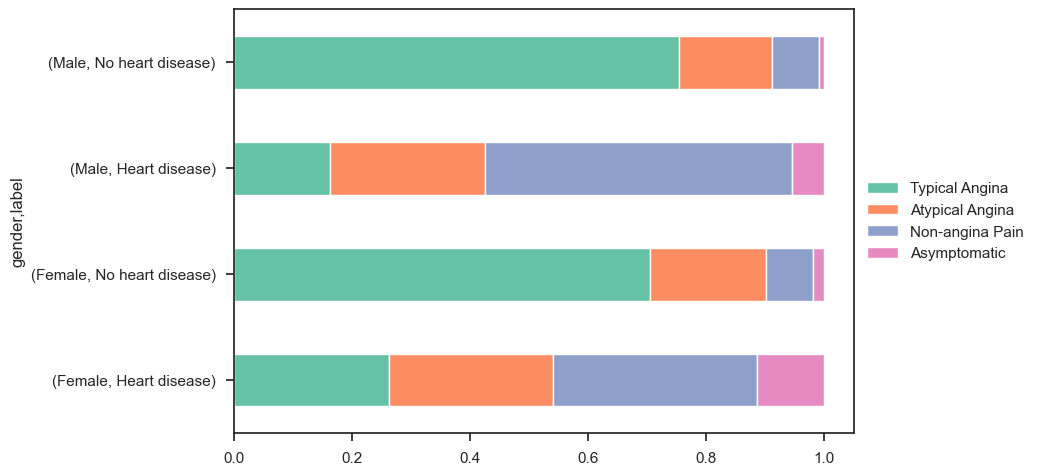
\includegraphics[width=\linewidth]{media/frequency-09-gender-paintype.png}
\end{figure}

\begin{figure}
    \caption{Distribution of chest pain type classification grouping by age groups}\label{frequency-paintype-agegroup-percent}
    \centering
    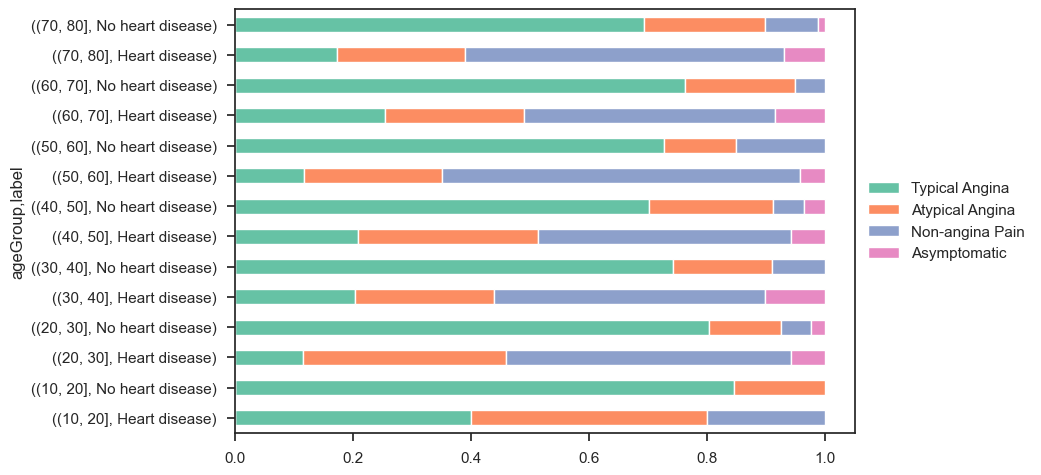
\includegraphics[width=\linewidth]{media/frequency-10-agegroup-paintype.png}
\end{figure}

\subsubsection{Feature: Exercise-induced angina}

This feature shows whether the patients suffered from an exercise-induced angina. Figures \ref{frequency-exerciseangina-gender-percent}
and \ref{frequency-exerciseangina-agegroup-percent} don't show any clear correlation between this feature
and heart disease.

\begin{figure}
    \caption{Distribution of exercise-induced angina grouping by gender}\label{frequency-exerciseangina-gender-percent}
    \centering
    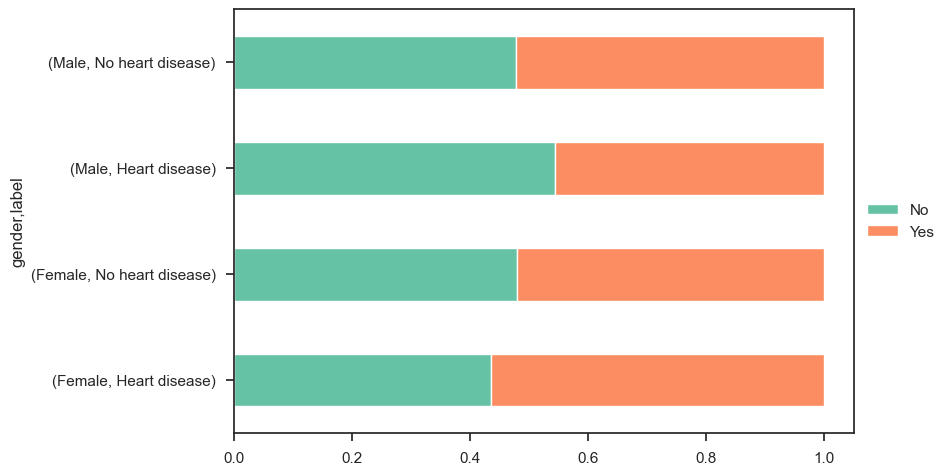
\includegraphics[width=\linewidth]{media/frequency-11-gender-exerciseangina.png}
\end{figure}

\begin{figure}
    \caption{Distribution of exercise-induced angina grouping by age groups}\label{frequency-exerciseangina-agegroup-percent}
    \centering
    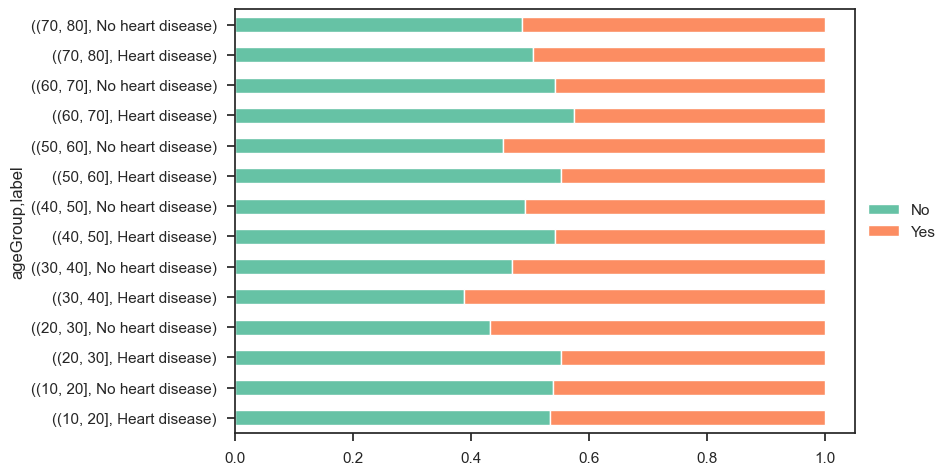
\includegraphics[width=\linewidth]{media/frequency-12-agegroup-exerciseangina.png}
\end{figure}

\subsection{Data spread and variability}

In this section we use measures of dispersion to analyse the data spread and variability across each feature.

\subsubsection{Feature: Oldpeak}

\begin{figure}
    \caption{Measures of dispersion for oldpeak grouping by age and gender}\label{boxplot-oldpeak-age}
    \centering
    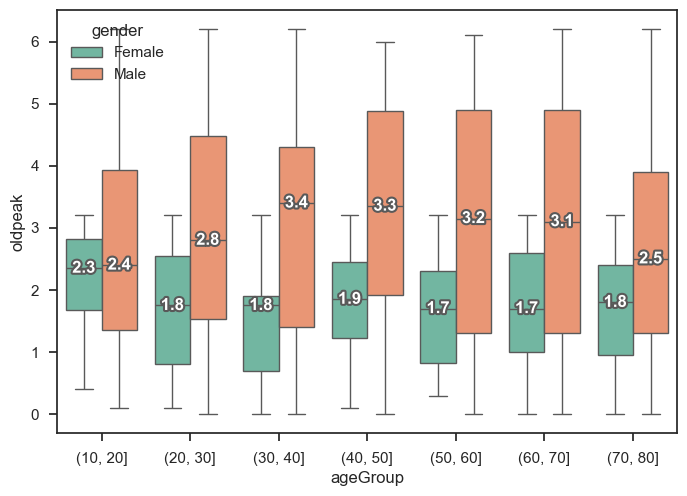
\includegraphics[width=\linewidth]{media/boxplot-01-agegroup-gender-oldpeak.png}
\end{figure}

\begin{figure}
    \caption{Measures of dispersion for oldpeak grouping by gender}\label{boxplot-oldpeak-gender}
    \centering
    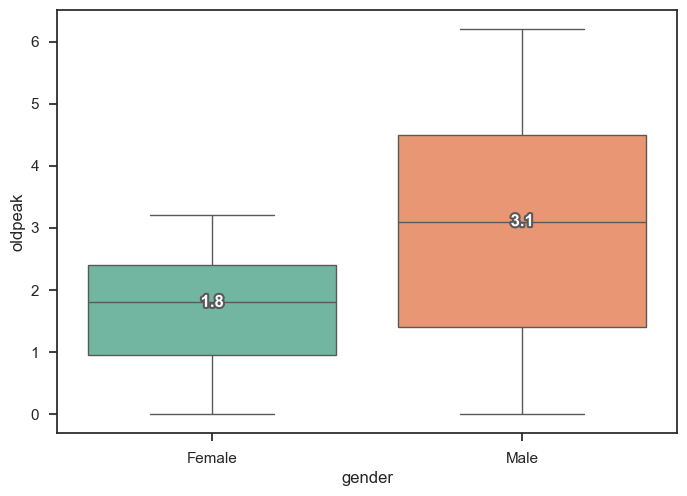
\includegraphics[width=\linewidth]{media/boxplot-02-gender-oldpeak.png}
\end{figure}

\subsubsection{Feature: Maximum heart rate achieved}

\begin{figure}
    \caption{Measures of dispersion for maximum resting heart rate grouping by age and gender}\label{boxplot-heartrate-age}
    \centering
    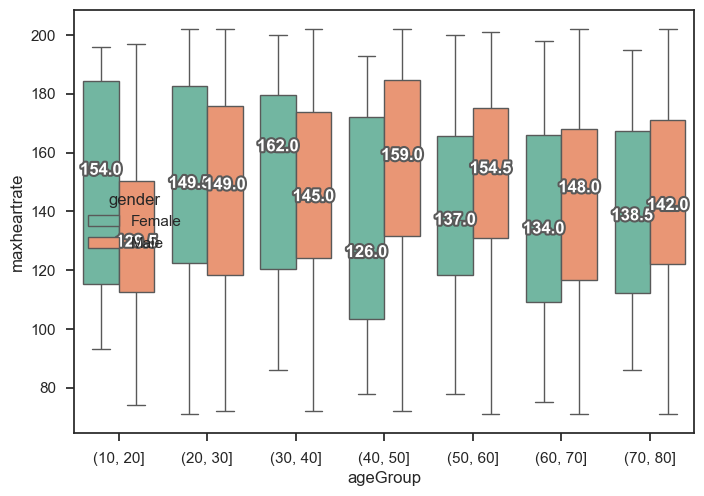
\includegraphics[width=\linewidth]{media/boxplot-03-agegroup-gender-heartrate.png}
\end{figure}

\begin{figure}
    \caption{Measures of dispersion for maximum resting heart rate grouping by gender}\label{boxplot-heartrate-gender}
    \centering
    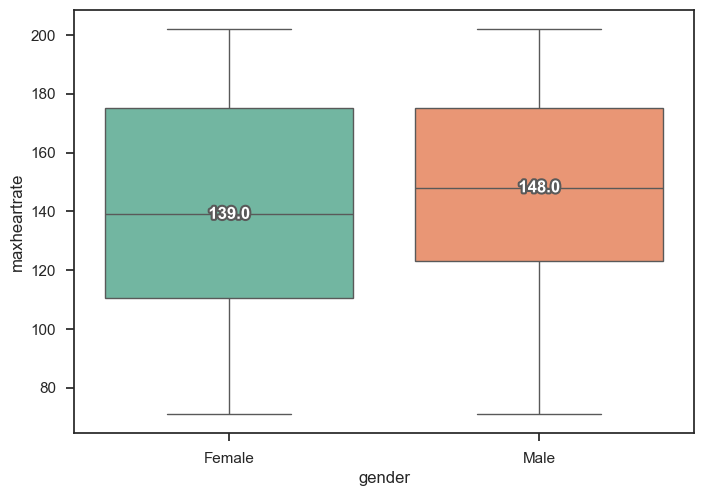
\includegraphics[width=\linewidth]{media/boxplot-04-gender-heartrate.png}
\end{figure}

\subsubsection{Feature: Serum cholesterol}

\begin{figure}
    \caption{Measures of dispersion for serum cholesterol grouping by age and gender}\label{boxplot-cholesterol-age}
    \centering
    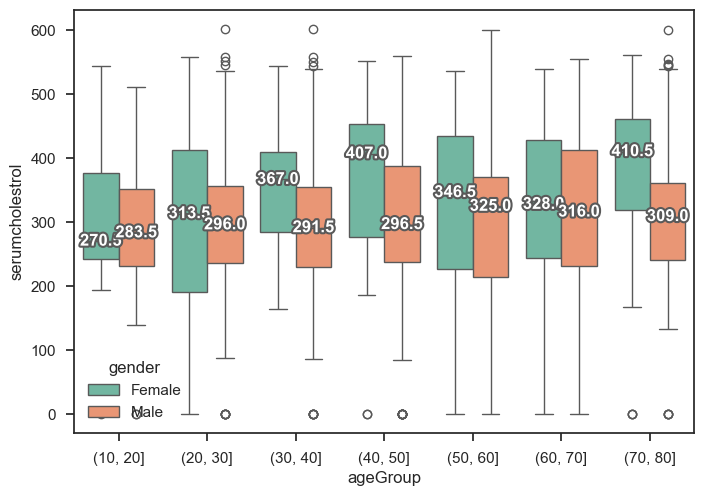
\includegraphics[width=\linewidth]{media/boxplot-05-agegroup-gender-cholesterol.png}
\end{figure}

\begin{figure}
    \caption{Measures of dispersion for serum cholesterol grouping by gender}\label{boxplot-cholesterol-gender}
    \centering
    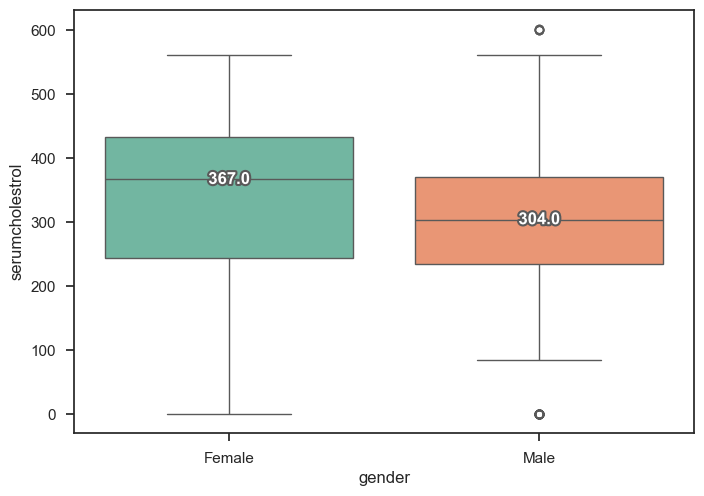
\includegraphics[width=\linewidth]{media/boxplot-06-gender-cholesterol.png}
\end{figure}

\subsubsection{Feature: Resting blood pressure}

\begin{figure}
    \caption{Measures of dispersion for resting blood pressure grouping by age and gender}\label{boxplot-bp-age}
    \centering
    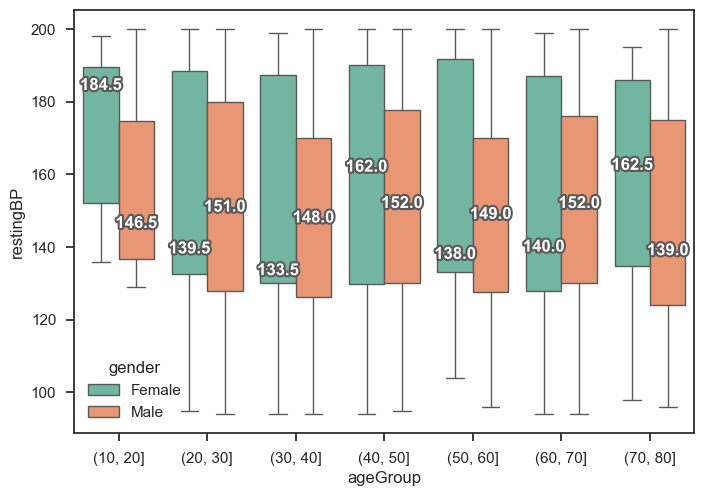
\includegraphics[width=\linewidth]{media/boxplot-07-agegroup-gender-bp.png}
\end{figure}

\begin{figure}
    \caption{Measures of dispersion for resting blood pressure grouping by gender}\label{boxplot-bp-gender}
    \centering
    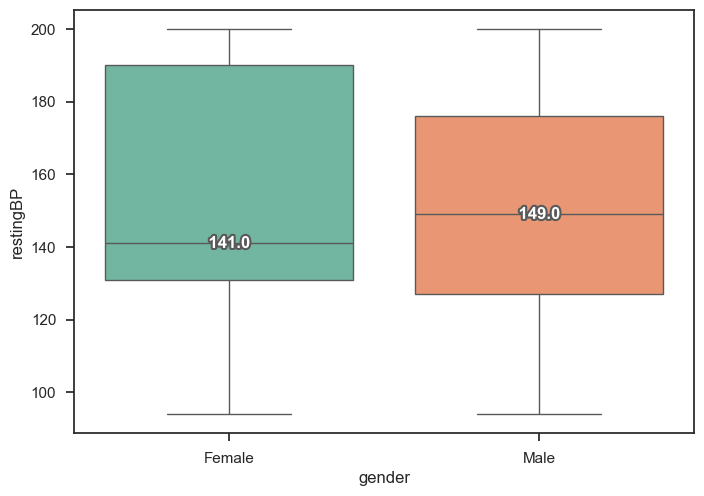
\includegraphics[width=\linewidth]{media/boxplot-08-gender-bp.png}
\end{figure}


\subsection{Correlation analysis}

\begin{figure}
    \caption{Correlation matrix}\label{correlation-matrix}
    \centering
    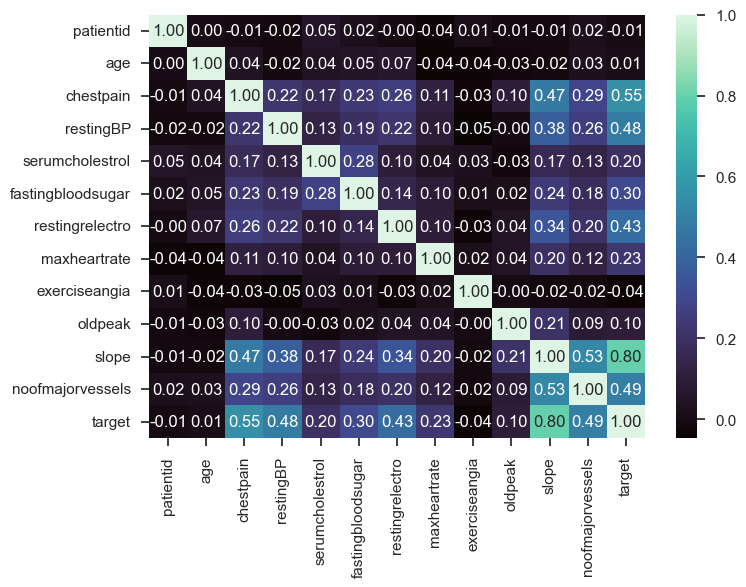
\includegraphics[width=\linewidth]{media/correlation-matrix.png}
\end{figure}